\documentclass{beamer}
\usetheme{Boadilla}
\usepackage[utf8]{inputenc}
\usepackage[polish]{babel}
\usepackage[T1]{fontenc}
\usepackage{hyperref}
\usepackage{listings}

\title{\textbf{Wyszukiwanie geometryczne -- przeszukiwanie obszarów ortogonalnych}}
\subtitle{\textit{quadtree} oraz \textit{kd-drzewa}}
\author{Stanisław Łenyk, Jerzy Wilczek}
\institute{Algorytmy geometryczne -- projekt}
\date{Styczeń 2021}


\begin{document}

\begin{frame}
    \titlepage
\end{frame}

\begin{frame}{Plan prezentacji}
    \tableofcontents
\end{frame}

\section{Przedstawienie problemu}

\begin{frame}{Wyszukiwanie geometryczne -- ogólne sformułowanie}
    Problem zdefiniowany jest następująco -- otrzymujemy na wejściu następujące dane:
    \begin{description}
        \item[P] Zbiór punktów
        \item[R] Region -- obszar, np. prostokąt, okrąg \textit{Uwaga: możemy dostać wiele zapytań w formie różnych regionów, ma to kluczowe znaczenie dla konstrukcji struktur danych odpowiednich do rozwiązania problemu}
    \end{description}
    \pause
    Na podstawie tych danych wejściowych musimy wyznaczyć
    \begin{description}
        \item[$P_R$] Podzbiór zbioru wszystkich punktów, taki, że $p \in P_R \iff p \in P \land p \in R$
    \end{description}
    \pause
    Należy więc stworzyć strukturę danych, która konstruuje się jak najszybciej, jak najszybciej odpowiada na zapytania i jak najszybciej aktualizuje się po zmianie w zbiorze $P$ (ostatnie tylko w pewnych sformułowaniach problemu) 
\end{frame}

\begin{frame}{Wyszukiwanie geometryczne -- wyszczególnienie problemu}
    W naszym projekcie rozważaliśmy wyszukiwanie geometryczne w przypadku, kiedy:
    \begin{itemize}
        \item<2-> regiony $R$ zawsze są prostokątami
        \item<3-> zbiór $P$ jest stały w czasie działania całego algorytmu
    \end{itemize}
\end{frame}

\section{Podejście pierwsze -- \textit{quadtree}}

\begin{frame}{Idea podziału przestrzeni w \textit{quadtree}}
Rekursywny podział na ćwiartki i odpowiednie przyporządkowywanie do każdej z nich zbioru danych wejściowych
\begin{figure}
    \centering
    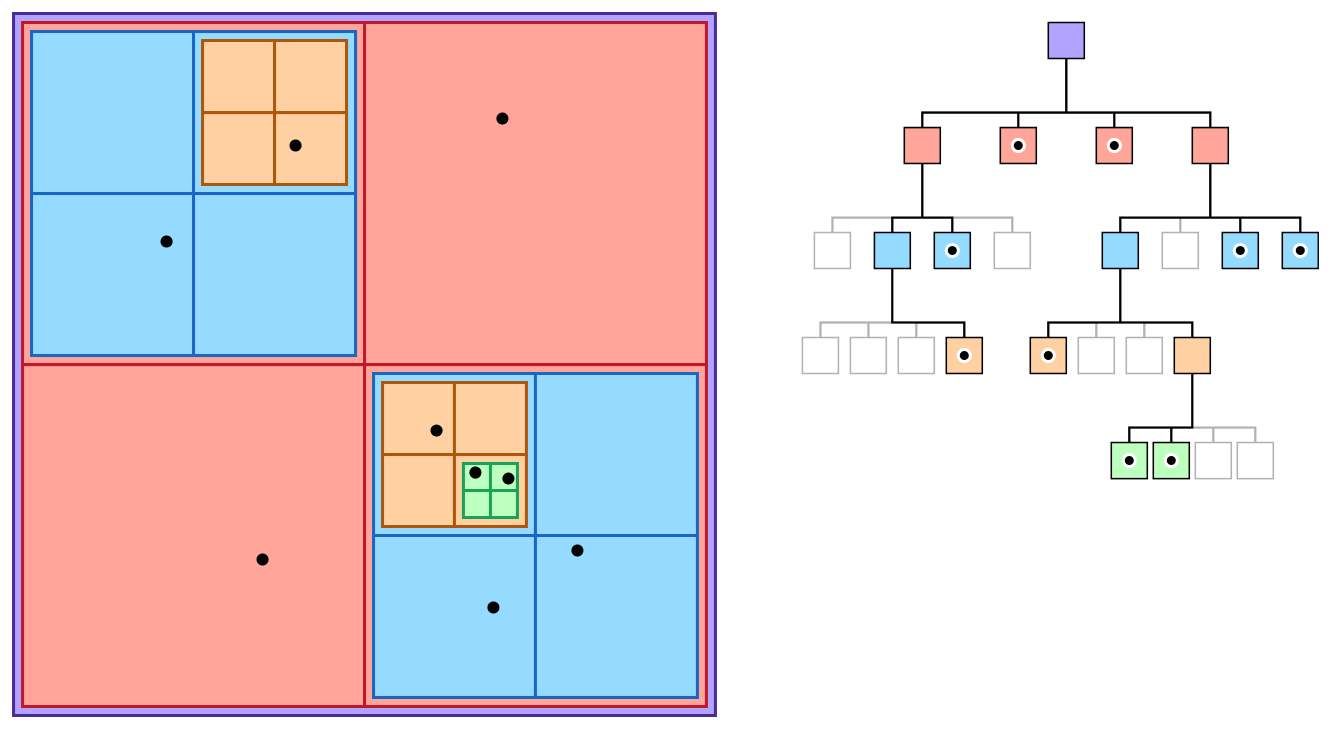
\includegraphics[width=\linewidth]{quadtree_image.png}
    \label{fig:quadtre}
\end{figure}

\end{frame}

\begin{frame}{\textit{quadtree} -- opis struktury}
    \textit{quadtree} (pol. \textit{drzewo ćwiartkowe, drzewo czwórkowe} jest drzewiastą strukturą, w której:
    \begin{itemize}
        \item <2-> każdy \textbf{wierzchołek} odpowiada za pewien obszar płaszczyzny
        \item <3-> każdy \textbf{wierzchołek} posiada maksymalnie czworo potomków
        \item <4-> każdy \textbf{potomek} odpowiada za ćwiartkę (NE, NW, SW, SE) obszaru swojego rodzica
        \item <5-> każdy \textbf{liść} odpowiada za dokładnie jeden punkt na płaszczyźnie
    \end{itemize}
\end{frame}

\begin{frame}{\textit{quadtree} -- złożoność obliczeniowa}
Budowanie drzewa -- $O(hn)$, h - wysokość drzewa

Na każdym poziomie drzewa punkty dzielone są na cztery części

Zapytanie -- $O(hk)$, k - liczba liści odpowiedzialnych za obszary posiadające przecięcie z zadanym
    
\end{frame}

\section{Podejście drugie -- \textit{kd-drzewa}}

\begin{frame}{\textit{kd-drzewa} -- opis struktury}
    kd-drzewa (k-wymiarowe drzewa) opierają się na koncepcie zbudowania drzewa podobnego do BST, w którym:
    \begin{itemize}
        \item<2-> \textbf{liście} przechowują po jednym punkcie
        \item<3-> \textbf{węzły inne niż liście} (włącznie z korzeniem) dzielą obszar, za który są odpowiedzialne na dwie części -- przechowują:
        \begin{itemize}
            \item<4-> \textit{wymiar podziału} -- wymiar, w którym przeprowadzony jest podział, np. równolegle do osi OX w dwóch wymiarach lub wzdłuż płaszczyzny prostopadłej do osi OY w trzech wymiarach
            \item<5-> \textit{współrzędną podziału} -- wartość taką, że punkty o współrzędnej w \textit{wymiarze podziału} mniejszej od niej lądują w lewym dziecku węzła, a większej -- w prawym
        \end{itemize}
    \end{itemize}
\end{frame}

\begin{frame}{\textit{kd-drzewa} -- wybieranie \textit{wymiaru podziału}}
    Jak wybrać wymiar podziału dla węzła?
    Dwa podejścia:
    \begin{itemize}
        \item<2-> wybieranie wymiarów na zmianę w cyklu -- prostsze w implementacji, szybsza konstrukcja drzewa, gorsza struktura drzewa (wolniejsze odpowiadanie na zapytania)
        \item<3-> wybieranie wymiaru, w którym największa różnica w odległości jest największa spośród wszystkich wymiarów -- tylko minimalnie trudniejsze w implementacji, wolniejsza konstrukcja drzewa, lepsza struktura drzewa (szybsze odpowiadanie na zapytania)
    \end{itemize}
    \pause
    W naszej implementacji zdecydowaliśmy się na opcję drugą.
\end{frame}

\begin{frame}{\textit{kd-drzewa} -- wybieranie \textit{współrzędnej podziału}}
    Aby zapewnić głębokość drzewa rzędu $O(log(n))$ jako współrzędną podziału wybieramy medianę względem danego wymiaru.\\
    \pause
    \begin{block}{Spostrzeżenie}
        Znalezienie mediany w każdym węźle niebędącym liściem jest jednym z najbardziej kosztownych kroków konstrukcji drzewa
    \end{block}
\end{frame}

\begin{frame}{\textit{kd-drzewa} -- problem znalezienia mediany}
    Możliwe rozwiązania problemu ze znalezieniem mediany:
    \begin{itemize}
        \item<2-> prosty w implementacji algorytm oparty na posortowaniu punktów działający w złożoności $O(nlog(n))$
        \item<3-> trudny w implementacji algorytm znajdujący medianę w czasie $O(n)$
        \item<4-> podejście alternatywne:
        \begin{itemize}
            \item<5-> ustalamy pewną stałą ilość punktów $m$, np. 1000
            \item<5-> jeśli w węźle jest mniej niż $m$ punktów obliczamy medianę przy użyciu prostego algorytmu
            \item<5-> jeśli w węźle jest więcej niż $m$ punktów losowo wybieramy $m$ z nich i to z tych punktów obliczamy medianę
        \end{itemize}
    \end{itemize}
    \onslide<5->{
        Alternatywne podejście pozwala na obliczenie zbliżonej do optymalnej \textit{współrzędnej podziału} w złożoności $O(1)$ przy zachowaniu oczekiwanej głębokości drzewa $O(log(n))$. \textbf{Wada:} pesymistyczna głębokość drzewa większa niż $O(log(n))$.
    }\\
    \onslide<6->{W naszej implementacji zdecydowaliśmy się na opcję trzecią.}
\end{frame}

\begin{frame}[fragile]{\textit{kd-drzewa} -- algorytm konstrukcji drzewa}
    Skoro mamy już sposoby na wyznaczenie wszystkich wartości służących do podziału, możemy zbudować drzewo, np. w taki przykładowy sposób
    \pause
    \begin{semiverbatim}
    buildSubtree(points):
        if points.length == 1
            return leaf(points)
        this.dimension = chooseDivisionDimension(points)
        this.median = calculateMedian(points, this.dimension)
        this.left = buildSubtree(
            \{p in P: p[this.dimension] <= this.median\}
        )
        this.right = buildSubtree(
            \{p in P: p[this.dimension] > this.median\}
        )
        return this
    \end{semiverbatim}
\end{frame}

\begin{frame}{\textit{kd-drzewa} -- złożoność obliczeniowa konstruowania struktury}
    Dla każdego poziomu w drzewie wykonujemy $O(n)$ operacji -- tyle zajmuje podział punktów między potomne węzły. Zakładając optymalną wysokość drzewa $O(log(n))$ całościowa złożoność obliczeniowa wynosi $O(nlog(n))$
\end{frame}

\begin{frame}[fragile]{\textit{kd-drzewa} -- przeszukiwanie drzew}
    W porównaniu z konstruowaniem drzewa przeszukiwanie go jest prostszą czynnością. Niech \texttt{region(v)} oznacza region, za którego przechowywanie odpowiedzialny jest wierzchołek \texttt{v}
    \begin{semiverbatim}
    KDSearch(v, R):
        if v.is_leaf and region(v).inside(R)
            return v
        if region(v).inside(R)
            return v.all_leaves_in_subtree
        result = \{\}
        if region(v.left).intersects(R)
            result.add(KDSearch(v.left, R))
        if region(v.right).intersects(R)
            result.add(KDSearch(v.right, R))
        return result
    \end{semiverbatim}
\end{frame}

\begin{frame}{\textit{kd-drzewa} -- jak wyznaczać \texttt{region(v)}}
    Są dwie możliwości na wyznaczanie \texttt{region(v)}
    \begin{itemize}
        \item przechowywać tę informację w każdym wierzchołku
        \item obliczać ją dynamicznie w trakcie przechodzenia po drzewie
    \end{itemize}
    W naszej implementacji wybraliśmy pierwszą opcję.
\end{frame}

\begin{frame}{\textit{kd-drzewa} -- złożoność obliczeniowa wyszukiwania}
    Złożoność obliczeniowa przeszukiwania \textit{kd-drzewa} wynosi $O(\sqrt{n} + k)$, gdzie $n$ to ilość punktów w drzewie, a $k$ to ilość punktów w wyjściu. Udowodnijmy najpierw, że każda pionowa lub pozioma prosta przecina $O(\sqrt{n})$ obszarów
    \begin{enumerate}
            \item<2-> ilość obszarów przecinana przez prostą na danym poziomie drzewa zwiększa się dwukrotnie co drugi poziome zagłębienia -- w jednym wymiarze podziału przecinane jest jedno z dzieci, w drugim dwa 
            \item<3-> w takim razie ilość obszarów przecięta przez prostą zdominowana jest przez obszary na najniższym piętrze z uwagi na wzrost wykładniczy
            \item<4-> drzewo jest zrównoważone -- $O(log(n))$ poziomów, więc ilość przecięć na najniższym poziomie jest równa $O(2^{log(n)/2}) = O(2^{log\sqrt{n}}) = O(\sqrt{n})$
    \end{enumerate}
\end{frame}

\begin{frame}{\textit{kd-drzewa} -- złożoność obliczeniowa wyszukiwania}
     \begin{enumerate}
        \item<1-> Złożoność niewynikająca z rozmiaru wyjścia jest taka jak ilość odwiedzonych obszarów, czyli taka jak ilość obszarów przeciętych przez prostokąt.
        \item<2-> Obszary znajdujące się w całości wewnątrz prostokąta natychmiast kończą swoje wywołanie, więc złożoność zdominowana jest przez ilość obszarów przeciętych przez boki prostokąta.
        \item<3-> Każda pionowa lub pozioma prosta przecina $O(\sqrt{n})$ obszarów.
        \item<4-> Prostokąt ma 4 boki, więc przecinają one $O(4\sqrt{n}) = O(\sqrt{n})$ obszarów
    \end{enumerate}
\end{frame}

\section{Zastosowanie \textit{quadtree} i \textit{kd-tree}}
\begin{frame}{Zastosowanie \textit{quadtree} i \textit{kd-tree}}
    \begin{itemize}
        \item kompresja obrazów
        \item wykrywanie kolizji w grach komputerowych
    \end{itemize}
\end{frame}

\section{Bibliografia}
\begin{frame}{Bibliografia}
\begin{enumerate}
    \item dr inż Barbara Głut \textit{Wykład -- wyszukiwanie geometryczne}
    \item Robert Bembenik \textit{Metody eksploracji danych z systemów informacji przestrzennej}, październik 2006
\end{enumerate}
\end{frame}

\end{document}